\documentclass{standalone}
\usepackage{tikz}
\usetikzlibrary{patterns, angles}

\begin{document}
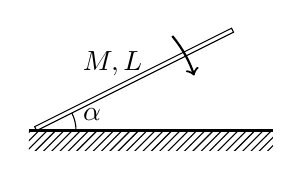
\begin{tikzpicture}
	\coordinate (A) at (0, 0);
    \coordinate (B) at (3, 0);
    \coordinate (C) at (2.5, 1.25);
           
	\draw [draw=none, pattern=north east lines] (3,0) rectangle (-0.1,-0.25);
	\draw [thick] (-0.1,0) -- (3,0);
	\draw (0,0) -- (2.5,1.25) -- (2.475, 1.3) node [left=43pt, below=5pt]{$M,L$}-- (-0.025, 0.05) -- cycle;
	\pic [draw, -, angle eccentricity=1.5] {angle = B--A--C};
	\node [right=20pt, above] at (A) {$\alpha$};
	\draw [thick, <-] (2, 0.7) arc (18:40:1.5);
	\end{tikzpicture}
\end{document}